\section*{Introdução}

No âmbito da unidade curricular de Administração de Redes, implementamos a rede emulada descrita na figura 1.\\
\begin{figure}[h]
\centering
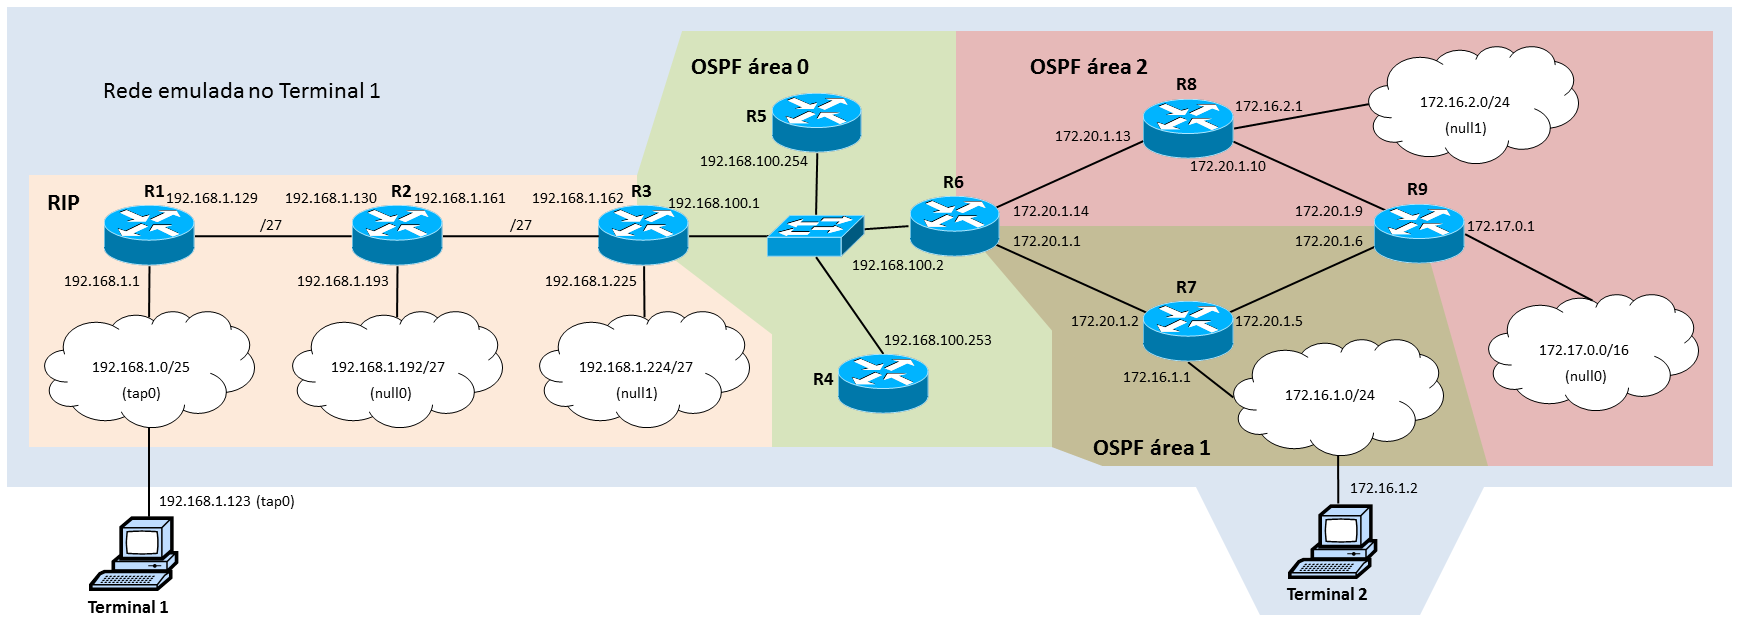
\includegraphics[width=1\textwidth, height=0.33\textheight]{rede-emulada.png}
\label{fig:rede emulada}
\caption{Rede emulada implementada na aula.}
\end{figure}
\\
Na rede emulada os \emph{routers} utilizados na simulação são da série 7200, o terminal 2 é um \emph{router} que funciona como se fosse um terminal.
Os terminais, terminal 1 e 2, usam como \emph{default gateway} o \emph{router} da rede à qual estão ligados, \emph{router} 1 e 7, respetivamente.\\
O \emph{router} R3 corre RIP em duas interfaces, (192.168.1.225 e 192.168.1.162), e OSPF numa outra, (192.168.100.1). Este \emph{router} redistribui no OSPF as rotas aprendidas pelo RIP e vice-versa.
